\documentclass{beamer}
\usepackage{tikz}
\usepackage{hyperref}
\usepackage{bm}
\usepackage{booktabs}       % professional-quality tables
\usetheme{metropolis}
\usepackage[utf8]{inputenc}
\usepackage[english]{babel}
\usepackage[T1]{fontenc}
\usepackage{helvet}
\usepackage{amsmath,amsfonts} % Math packages
\usepackage{mathtools}
\usepackage{bbm}
\usepackage{tcolorbox}
\usepackage{standalone}
\usepackage{pgfplots}  % Plots in Latex

% Plotting settings for the introduction plots
\pgfplotsset{width=7cm,compat=1.8}
\pgfplotsset{%
  colormap={whitered}{color(0cm)=(white);
  color(1cm)=(orange!75!red)}
}


%-------------------------------------------------------
% DEFFINING AND REDEFINING COMMANDS
%-------------------------------------------------------
\newsavebox{\genericfilt}
\savebox{\genericfilt}{%

\begin{tikzpicture}[font=\small, >=stealth,yscale=0.15,xscale=0.1]
  % define normal distribution function 'normaltwo'
  \def\normaltwo{\x,{exp((-(\x)^2)/0.5)}}
  \draw[line width=0.25mm,domain=-1.7:1.7] plot (\normaltwo);
\end{tikzpicture}%
}

\newsavebox{\genericfiltLarge}
\savebox{\genericfiltLarge}{%

\begin{tikzpicture}[font=\small, >=stealth,yscale=0.25,xscale=0.2]
  % define normal distribution function 'normaltwo'
  \def\normaltwo{\x,{exp((-(\x)^2)/0.5)}}
  \draw[line width=0.25mm,domain=-1.7:1.7] plot (\normaltwo);
\end{tikzpicture}%
}

% colored box for highlighting
\newtcbox{\martinbox}[1][red]{
  on line, 
  %arc=7pt,
  colback=#1!10!white,
  colframe=#1!50!black, 
  before upper={\rule[-3pt]{0pt}{10pt}},
  boxrule=0.5pt, 
  boxsep=0pt,
  left=6pt,
  right=6pt,
  top=2pt,
  bottom=2pt
}

\newtcbox{\martintitlebox}[1][red]{
  %on line, 
  %arc=7pt,
  colback=#1!10!white,
  colframe=#1!50!black, 
  before upper={\rule[-3pt]{0pt}{10pt}},
  boxrule=0pt, 
  boxsep=0pt,
  left=6pt,
  right=6pt,
  top=6pt,
  bottom=6pt
}

% Load definitions
%\newtcolorbox{titlebox}{colback=background,colframe=CBBlue,coltext=gray}
\newtcolorbox{defbox}{colback=white,colframe=gray,coltext=black}

\newcommand{\Categorical}{\ensuremath{\mathcal{C}at}}
\newcommand\Beta{\ensuremath{\mathcal{B}eta}}
\newcommand\Bernoulli{\ensuremath{\mathcal{B}ern}}
\newcommand{\Dirichlet}{\ensuremath{\mathcal{D}ir}}
\newcommand{\Normal}{\ensuremath{\mathcal{N}}}
\newcommand{\Exponential}{\ensuremath{\mathcal{E}xp}}
\newcommand{\Poisson}{\ensuremath{\mathcal{P}oisson}}
\newcommand\DP{\ensuremath{\mathrm{DP}}}
\newcommand\GEM{\ensuremath{\mathrm{GEM}}}
\newcommand{\indpath}[2]{\mathbin{\mathcal{P}{\left(#1,#2\right)}}} % induced path
\newcommand{\indic}{\mathbbm{1}}
\newcommand{\diff}{\mathop{}\!\mathrm{d}}
\newcommand{\SPT}{\mathcal{T}}
\newcommand{\SPG}{\mathcal{C}}
\newcommand{\SPN}{\mathcal{S}}
\newcommand{\graph}{\mathcal{G}}
\newcommand{\ProductNode}{\mathsf{P}}
\newcommand{\ProductNodes}{\bm{\mathsf{P}}}
\newcommand{\SumNode}{\mathsf{S}}
\newcommand{\SumNodes}{\bm{\mathsf{S}}}
\newcommand{\Leaf}{\mathsf{L}}
\newcommand{\Leaves}{\bm{\mathsf{L}}}
\newcommand{\Node}{\mathsf{N}}
\newcommand{\Nodes}{\bm{\mathsf{N}}}
\newcommand{\Child}{\mathsf{C}}
\newcommand{\region}{\ensuremath{R}}
\newcommand{\partition}{\ensuremath{P}}
\newcommand{\regions}{\ensuremath{\mathbf{R}}}
\newcommand{\partitions}{\ensuremath{\mathbf{P}}}
\newcommand{\rg}{\ensuremath{\mathcal{R}}}

\newcommand{\X}{\mathbf{X}}
\newcommand{\data}{\mathcal{X}}
%\newcommand{\x}{\mathbf{x}}
\newcommand{\xn}{\mathbf{x}_{n}}
\newcommand{\xnd}{x_{n,d}}
\newcommand{\xd}{\mathbf{x}_{\cdot,d}}
\newcommand{\Y}{\mathbf{Y}}
\newcommand{\y}{\mathbf{y}}
\newcommand{\yd}{\mathbf{y}}
\newcommand{\ydp}{y_{d,\ProductNode}}
\newcommand{\yndp}{\mathbf{y_{\not{d},\ProductNode}}}
\newcommand{\ydP}{y_{d,\partition}}
\newcommand{\yndP}{\mathbf{y_{\not{d},\partition}}}
\newcommand{\yProduct}{\mathbf{y}_{\cdot,\ProductNode}}
\newcommand{\yPartition}{\mathbf{y}_{\cdot,\partition}}
\newcommand{\Z}{\mathbf{Z}}
\newcommand{\z}{\ensuremath{\mathbf{z}}}
\newcommand{\zn}{\ensuremath{\mathbf{z}_n}}
\newcommand{\zs}{\ensuremath{z_\SumNode}}
\newcommand{\zsn}{\ensuremath{z_{\SumNode,n}}}
\newcommand{\tld}{\ensuremath{\theta_{d,\Leaf}}}


\newcommand{\ks}{\mathbf{k}}
\newcommand{\Root}{\ensuremath{\mathbf{root}}}
\newcommand{\ch}{\ensuremath{\mathbf{ch}}}
\newcommand{\anc}{\ensuremath{\mathbf{anc}}}
\newcommand{\leaf}[1]{\mathbin{\mathbf{leaf}(#1)}} % leaf function
\newcommand{\leafs}[1]{\mathbin{\mathbf{leafs}(#1)}} % leaf function
\newcommand{\w}{w}
\newcommand{\vp}{\mathbf{v}}
\newcommand{\vps}{\mathbf{v}}
%\newcommand{\ws}{\mathbf{w}_{\SumNode}}
\newcommand{\wsc}{w_{\SumNode,\Child}}
\newcommand{\tp}{\mathbf{\theta}}
\newcommand{\val}{\ensuremath{\mathbf{val}}}
\newcommand{\scope}{\psi}
\newcommand{\cond}[2]{\mathbin{\left. #1\nonscript\;\middle|\nonscript\; #2 \right.}}
\newcommand{\cbar}{\,|\,}

\newcommand{\xnew}{\mathbf{x}^{*}}

\newcommand{\argmin}{\arg\!\min} % arg min
\newcommand{\argmax}{\arg\!\max} % arg max

\DeclareMathOperator*{\f}{\SPN(\xn \,|\, \phi)}
\DeclareMathOperator*{\fz}{\SPN(\bm \ast \,|\, \phi)}
\DeclareMathOperator*{\fy}{\SPN(\xn, \lambda_n \,|\, \phi)}
\DeclareMathOperator*{\fzy}{\SPN(\bm \ast, \lambda_n \,|\, \phi)}
\newcommand{\wa}{\w^{[0]}_{\gamma}}
\newcommand{\wb}{\w^{[1]}_{k}}
\newcommand{\wt}{\w^{(t)}_{k}}
\newcommand{\wjt}{\w^{(t)}_{j}}
\newcommand{\wjtt}{\w^{(t+1)}_{j}}
\newcommand{\wtt}{\w^{(t+1)}_{k}}
\newcommand{\wat}{\w^{[0](t)}_{\gamma}}
\newcommand{\wbt}{\w^{[1](t)}_{k}}
\newcommand{\wjbt}{\w^{[1](t)}_{j}}
\newcommand{\watt}{\w^{[0](t+1)}_{\gamma}}
\newcommand{\wbtt}{\w^{[1](t+1)}_{k}}


%-------------------------------------------------------
% INFORMATION IN THE TITLE PAGE
%-------------------------------------------------------

\title[Sum-Product Networks] { Learning Sum-Product~Networks }
\author { Martin Trapp }

\titlegraphic{
  \begin{picture}(0,0)
    \put(350,-200){\makebox(0,0)[rt]{
      
\includegraphics[width=2cm]{TU_Graz} \hspace*{1cm}~
    }}
  \end{picture}
}

\date{}

%-------------------------------------------------------
% THE BODY OF THE PRESENTATION
%-------------------------------------------------------

\begin{document}

%-------------------------------------------------------
% THE TITLEPAGE
%-------------------------------------------------------
\maketitle

%-------------------------------------------------------
% INTRODUCTION
%-------------------------------------------------------

% --
% Introduction on Probabilistic machine learning
% --
\section{Probabilistic Machine Learning}

\frame{
\begin{itemize}
    \item Machine learning: How can we make machines that learn from data?
    \item Probabilistic machine learning: How can we make machines that learn from data using tools from probability theory?
    \item Uncertainty is key to probabilistic machine learning and is expressed in all forms, e.g.~noise in the data, uncertainty over the predictions, uncertainty over the model.
\end{itemize}
}

\frame{
Example: How likely is a traffic jam on highway $X_1$ today?

\begin{itemize}
    \item today = Thursday = $Y = 4$.
    \item Traffic jam model: $\theta$ for all $\{X_i\}_{i=1}^n$ highways in the country.
    \item $p(X_1 = 1, Y = 4 \,|\, \theta) = \int_{X_2} \int_{X_3} \dots \int_{X_n} p(X_1 = 1, Y = 4, X_2 = x_2, X_3 = x_3, \dots, X_n = x_n \, | \, \theta)$
    \item \textbf{We need to be able to marginalise out $X_2, \dots, X_n$ to answer the query.}
\end{itemize}
}

\frame{
    \textbf{Problem:} Probabilistic inference task, such as marginalisation, are often intractable for interesting models.

\begin{table}
\centering
\begin{tabular}{lllll}
             & GANs & VAEs & Flows & SPNs  \\
Sampling     & Y    & Y    & Y     & Y      \\
Density      & N    & N/Y  & Y     & Y      \\
Marginals    & N    & N    & ?     & Y      \\
Conditionals & N    & N    & ?     & Y      \\
Moments      & N    & N    & ?     & Y      \\
MAP          & N    & N    & ?     & N/Y
\end{tabular}
\caption{Robert Peharz, Sum-Product Networks and Deep Learning: A Love Marriage. Talk at ICML, 2019.}
\end{table}
}


% --
% Introduction on Sum-Product Networks
% --
\section{Sum-Product Networks}

\frame{
\begin{itemize}
  \item Sum-product networks (SPNs)\footnote{\scriptsize H. Poon \& P. Domingos: Sum-product networks: A new deep architecture. In UAI, 2011.} is a class of general-purpose probabilistic machine learning models that admit tractable probabilistic inference.
  \item SPNs are a sub-class of so-called tractable probabilistic models or probabilistic circuits.
   \item A class of queries $Q$ on a class of models $M$ is tractable, iff for any query $q \in Q$ and model $m \in M$ the computational complexity is at most polynomial.
  \item SPNs admit many probabilistic inference tasks, such as marginalisation, in linear time in their representation size.
  \end{itemize}
}

\begin{frame}{What is a Sum-Product Network?}
\begin{itemize}
  \item Let $\X = \{X_1, \dots, X_D\}$ be set of $D$ random variables. 
  \item An SPN is a distribution over $\X$ defined as a 4-tuple $\SPN = (\graph, \scope, \w, \tp)$.
  \begin{itemize}
    \item $\graph$ is a computational graph.
    \item $\scope$ is a so-called scope function.
    \item $\w$ denotes the set of sum-weights and $\tp$ the set of leaf node parameters. 
  \end{itemize}
\end{itemize}
 \small This definition\footnote{\scriptsize M. Trapp et al.: Bayesian Learning of Sum-Product Networks. In NeurIPS, 2019.} is conceptually different to the original definitions as it disentangles the computational graph and the scope function.
\end{frame}

\begin{frame}{Computational Graph $\graph$}
 $\graph$ is a rooted connected directed acyclic graph (DAG), containing: sum ($\SumNode$), product ($\ProductNode$) and leaf nodes ($\Leaf$).

\begin{figure}
  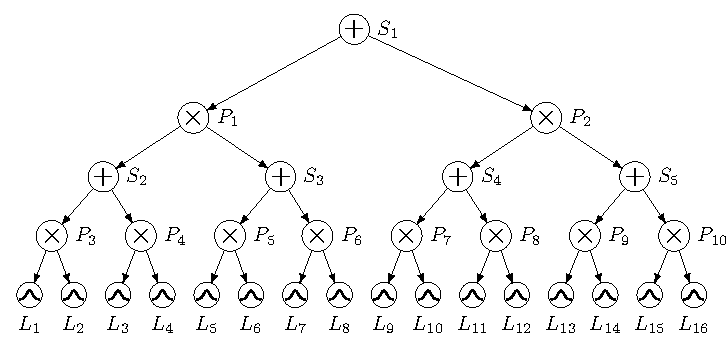
\includegraphics[width=\textwidth]{computation_graph}
  \caption{Example of a tree-shaped computational graph.}
\end{figure}
\end{frame}

\begin{frame}{Leaves $\Leaf$ in $\graph$}
 Leaf nodes are input nodes with arbitrary distribution, e.g.~Gaussian, Multinomial, variational autoencoder.\\[1em]
 
\tikzstyle{vertex}=[inner sep=0.01cm, circle, draw]
\begin{columns}
\begin{column}{.2\linewidth}
\end{column}
\begin{column}{.2\linewidth}
\begin{tikzpicture} [scale=0.5, auto,>=latex,transform shape]
   \node[draw=none](v01) at (1, 1.5) {};
   \node[draw=none](v02) at (-1, 1.5) {};
   \node[vertex](v1) at (0, 0) {\usebox{\genericfiltLarge}};
   \draw [->] (v01) -- (v1);
   \draw [->] (v02) -- (v1);
\end{tikzpicture}
\end{column}
\begin{column}{.4\linewidth}
$\Leaf(x) = p(x \cbar \tp_\Leaf)$
\end{column}
\begin{column}{.2\linewidth}
\end{column}
\end{columns}

\centering
\begin{figure}
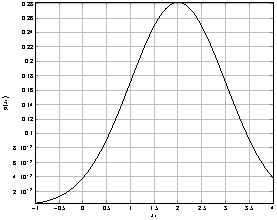
\includegraphics{leaf_distribution}
\end{figure}
\end{frame}

\begin{frame}{Product Nodes $\ProductNode$ in $\graph$}
Product nodes encode independence assumptions between sets of random variables.\\[1em]
 
 \tikzstyle{vertex}=[inner sep=0.01cm, circle, draw]
\begin{columns}
\begin{column}{.2\linewidth}
\end{column}
\begin{column}{.2\linewidth}
\begin{tikzpicture} [scale=0.5, auto,>=latex,transform shape]
   \node[draw=none](v01) at (1, 1.5) {};
   \node[draw=none](v02) at (-1, 1.5) {};
   \node[draw=none](v21) at (1, -1.5) {};
   \node[draw=none](v22) at (-1, -1.5) {};
   \node[vertex](v1) at (0, 0) {\huge$\bm\times$};
   \draw [->] (v01) -- (v1);
   \draw [->] (v02) -- (v1);
   \draw [->] (v1) -- (v21);
   \draw [->] (v1) -- (v22);
\end{tikzpicture}
\end{column}
\begin{column}{.4\linewidth}
$\ProductNode(x)  = \prod\limits_{\Child \in \ch(\ProductNode)} \Child(x)$
\end{column}
\begin{column}{.2\linewidth}
\end{column}
\end{columns}

\centering
\begin{figure}
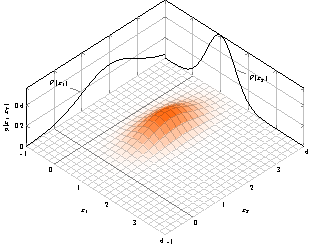
\includegraphics{product_distribution}
\end{figure}
\end{frame}

\begin{frame}{Sum Nodes $\SumNode$ in $\graph$}
Sum nodes\footnote{\scriptsize We assume that $\w_{\SumNode, \Child} \geq 0$ .} replace independence with conditional independence within the network.\\[1em]

\tikzstyle{vertex}=[inner sep=0.01cm, circle, draw]
\begin{columns}
\begin{column}{.2\linewidth}
\end{column}
\begin{column}{.2\linewidth}
\begin{tikzpicture} [scale=0.5, auto,>=latex,transform shape]
   \node[draw=none](v01) at (1, 1.5) {};
   \node[draw=none](v02) at (-1, 1.5) {};
   \node[draw=none](v21) at (1, -1.5) {};
   \node[draw=none](v22) at (-1, -1.5) {};
   \node[vertex](v1) at (0, 0) {\huge$\bm+$};
   \draw [->] (v01) -- (v1);
   \draw [->] (v02) -- (v1);
   \draw [->] (v1) -- (v21);
   \draw [->] (v1) -- (v22);
\end{tikzpicture}
\end{column}
\begin{column}{.4\linewidth}
$\SumNode(x)  = \sum\limits_{\Child \in \ch(\ProductNode)}  \w_{\SumNode, \Child}\Child(x)$
\end{column}
\begin{column}{.2\linewidth}
\end{column}
\end{columns}

\centering
\begin{figure}
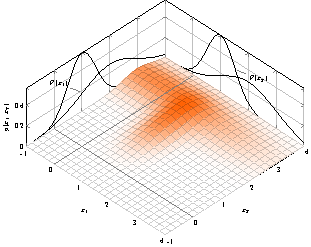
\includegraphics{sum_distribution}
\end{figure}
\end{frame}

\begin{frame}{Scope Function $\scope$}
$\scope$ is a function assigning each node $\Node$ in a sub-set of $\X$,\footnote{\scriptsize This sub-set is often referred to as the scope of a node.} and has to fulfil the following properties: 
\begin{defbox}
\begin{enumerate}
\item If $\Node$ is the root node, then $\scope(\Node) = \X$.
\item If $\Node$ is a sum or product, then $\scope(\Node) = \bigcup_{\Node' \in \ch(\Node)} \scope(\Node')$.
\item For each $\SumNode \in \SumNodes$ we have $\forall \Node, \Node' \in \ch(\SumNode)\colon \scope(\Node) = \scope(\Node')$ (\emph{completeness}) \footnote{\scriptsize Complete and decomposable SPNs are referred to as valid SPNs.}.
\item For each $\ProductNode \in \ProductNodes$ we have $\forall \Node, \Node' \in \ch(\ProductNode)\colon \scope(\Node) \cap \scope(\Node') = \emptyset$ (\emph{decomposability}).
\end{enumerate}
\end{defbox}
\end{frame}

\frame{
\begin{center}Example SPN $\SPN = (\graph, \scope, \w, \tp)$\end{center}
\begin{figure}
  \centering{
    \includestandalone[width=0.9\textwidth]{SPN}
    }
\end{figure}
After applying a scope function $\scope$  on $\graph$ we obtain the SPN. Most structure learners learn both in an entangled way.

\small Note that we define $\Leaf(x):=1$ for every $x$ if and only if $\scope(\Leaf) = \emptyset$.
}


\end{document}